\documentclass[11pt]{article}
\usepackage[margin=1in]{geometry}
\usepackage{amsmath,amssymb,amsthm}
\usepackage{graphicx}
\usepackage{microtype}
\usepackage[hidelinks]{hyperref}
\usepackage{enumitem}

\newtheorem{theorem}{Theorem}
\newcommand{\ellone}{\ell^1}
\newcommand{\elltwo}{\ell^2}
\newcommand{\supp}{\operatorname{supp}}
\newcommand{\R}{\mathbb{R}}

\title{Exact Noisy Support Cutoff Fails in Oversmoothing $\ell^1$ Regularization}
\author{Run \texttt{fa\_banach\_001} -- lane 1}
\date{27 August 2026}

\begin{document}
\maketitle

\noindent\textbf{Status.} Candidate counterexample, likely valid.  The result
disproves the exact support-localization route proposed in the source; it does
not disprove convergence rates or quantitative tail bounds.

\section{Source question and its precise reading}

Gerth and Hofmann consider oversmoothing $\ellone$ regularization when the
exact solution belongs to $\elltwo\setminus\ellone$.  In their final
discussion they describe an incomplete argument based on truncations
$P_nx^\dagger$ and state that the open problem is to show that ``the support
of the approximate solutions is not larger than this $n(\delta)$''
\cite[printed pp.~18--19]{GH2018}.  The source passage is reproduced below.

\clearpage
\begin{center}
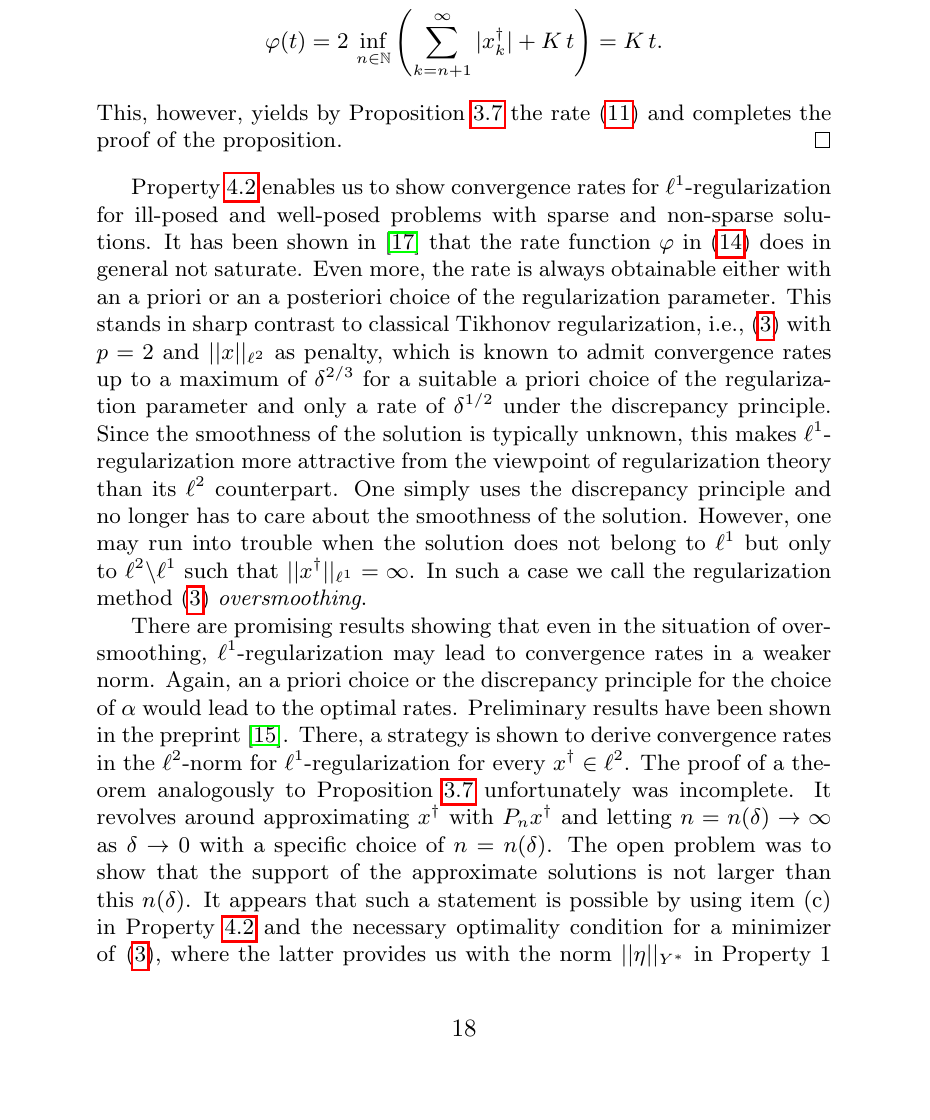
\includegraphics[width=0.78\textwidth]{figures/open_problem_crop_1.png}

\vspace{0.5em}
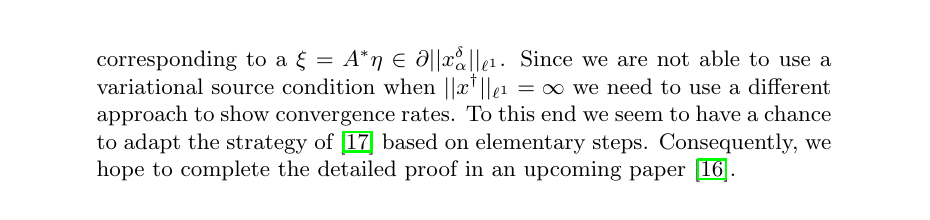
\includegraphics[width=0.78\textwidth]{figures/open_problem_crop_2.png}
\end{center}
\clearpage

The truncation argument needs the exact initial-segment localization
\begin{equation}\label{eq:cutoff}
  \supp(x_{\alpha}^{\delta})\subseteq\{1,\ldots,n(\delta)\},
  \qquad\text{equivalently}\qquad
  (I-P_{n(\delta)})x_{\alpha}^{\delta}=0.
\end{equation}
We show that \eqref{eq:cutoff} is false under the stated deterministic noise
model, already in the polynomial diagonal example used by the announced
follow-up paper \cite{GH2019}.

\section{Idea of the proof}

For a diagonal forward operator the $\ellone$-regularized minimizer is obtained
by coordinatewise soft thresholding.  The follow-up parameter scaling makes
the threshold in data coordinate $n+1$ smaller than the allowed noise amplitude
$\delta$: their ratio is at most a fixed constant divided by $\sqrt n$.
Placing the whole admissible noise vector in coordinate $n(\delta)+1$ therefore
forces that coordinate to survive thresholding.  Exact support cutoff is thus
too brittle for worst-case deterministic noise; a tail-norm estimate is the
appropriate replacement.

\section{Counterexample}

Fix $\beta>0$ and $\eta\in(1/2,1]$.  On $\elltwo$ let
\[
  Ae_k=\sigma_ke_k,\qquad \sigma_k=k^{-\beta},
  \qquad x_k^\dagger=k^{-\eta},
  \qquad y=Ax^\dagger.
\]
Then $A$ is compact and injective, while
$x^\dagger\in\elltwo\setminus\ellone$.  Put
\[
  T_m=\|(I-P_m)x^\dagger\|_2,
  \qquad
  \varphi(\delta)=\min_{m\geq1}\left(\frac{\delta}{\sigma_m}+T_m\right),
\]
and choose any minimizing index $n(\delta)$.  This is the prototype rate and
truncation index of \cite[Section~4]{GH2019}.  For a fixed constant
$c_\alpha>0$, take the same a priori scaling
\begin{equation}\label{eq:alpha}
  \alpha(\delta)=
  \frac{c_\alpha\delta^2}
       {\sqrt{n(\delta)}\,\varphi(\delta)}.
\end{equation}

For data $y^\delta$, let $x_\alpha^\delta$ minimize
\begin{equation}\label{eq:tikh}
  \frac12\|Ax-y^\delta\|_2^2+\alpha\|x\|_1
  \quad\text{over }x\in\elltwo.
\end{equation}

\begin{theorem}\label{thm:main}
For every fixed $c_\alpha>0$ and every sufficiently small $\delta>0$, there
is admissible data $y^\delta$ with $\|y^\delta-y\|_2=\delta$ for which
\[
  n(\delta)+1\in\supp(x_\alpha^\delta).
\]
Consequently, the exact support cutoff \eqref{eq:cutoff} fails even in this
diagonal oversmoothing model.
\end{theorem}

\begin{proof}
First, $n(\delta)\to\infty$ as $\delta\downarrow0$.  Indeed, for each fixed
$M$, $T_M>0$.  Choose $m>M$ with $T_m<T_M/2$ and then choose $\delta$ so small
that $\delta/\sigma_m<T_M/2$.  The objective at $m$ is then smaller than its
limit $T_M$ at every index at most $M$, after decreasing $\delta$ once more if
needed.  Thus no bounded sequence of indices can minimize for arbitrarily small
$\delta$.

Write $n=n(\delta)$.  Since
$\varphi(\delta)\geq\delta/\sigma_n$, equation \eqref{eq:alpha} gives
\begin{equation}\label{eq:key}
  \frac{\alpha}{\delta\sigma_{n+1}}
  \leq
  \frac{c_\alpha}{\sqrt n}\frac{\sigma_n}{\sigma_{n+1}}
  =\frac{c_\alpha}{\sqrt n}\left(1+\frac1n\right)^\beta
  \leq \frac{c_\alpha 2^\beta}{\sqrt n}.
\end{equation}
The right-hand side tends to zero.  Hence
$\alpha<\delta\sigma_{n+1}$ for all sufficiently small $\delta$.

Now set
\[
  y^\delta=y+\delta e_{n+1}.
\]
This data vector has exactly the allowed noise norm.  Since \eqref{eq:tikh}
decouples in the diagonal basis, its unique minimizer is given by soft
thresholding:
\[
  (x_\alpha^\delta)_k
  =S_{\alpha/\sigma_k^2}
    \left(\frac{y_k^\delta}{\sigma_k}\right),
  \qquad
  S_\lambda(t)=\operatorname{sgn}(t)(|t|-\lambda)_+.
\]
At $k=n+1$ all terms are positive, and therefore
\[
  (x_\alpha^\delta)_{n+1}
  =x_{n+1}^\dagger+\frac{\delta}{\sigma_{n+1}}
      -\frac{\alpha}{\sigma_{n+1}^2}>0,
\]
where the last inequality follows already from
$\delta\sigma_{n+1}>\alpha$.  Thus the minimizer has nonzero support strictly
beyond $n(\delta)$, proving the claim.
\end{proof}

\section{Relation to the follow-up literature}

The announced follow-up \cite{GH2019} restricts the general program to compact
diagonal operators.  Its noisy-data argument does not assert exact vanishing
beyond $n(\delta)$; instead Lemma~4.4 estimates
$\|(I-P_{n(\delta)})x_\alpha^\delta\|_2$.  Theorem~\ref{thm:main} explains why
this weakening is necessary under worst-case deterministic noise.  The
counterexample does not challenge that quantitative estimate or the resulting
convergence-rate theorem.

\section{Verification and novelty bounds}

The script \texttt{code/verify\_counterexample.py} evaluates the exact
soft-threshold formula for $\beta=1$, $\eta=3/4$, $c_\alpha=10$, and five noise
levels from $10^{-4}$ to $10^{-6}$.  In all cases the coefficient at
$n(\delta)+1$ is positive.  This computation is only a sanity check; the proof
above is analytic.

A bounded search through 27 August 2026 used arXiv, the exact source and
follow-up titles, the authors' publication page, the exact source phrase, and
combinations of ``support'', ``noise'', ``counterexample'', ``correction'',
``erratum'', and $n_{\mathrm{inf}}$.  It found the 2019 follow-up and later
oversmoothing work, but no explicit record of this counterexample or an erratum
addressing the exact cutoff.  The novelty claim is therefore only that the
argument appears unrecorded within this bounded search.

\section{Limitations and review recommendation}

The result addresses support \emph{localization} in the first $n(\delta)$
coordinates, the interpretation required to make the $P_n$ tail vanish.  It
does not rule out a statement only about the cardinality of the support.  A
reviewer should first confirm this interpretation of the source wording; after
that, the only substantive checks are the soft-threshold formula and estimate
\eqref{eq:key}.

\begin{thebibliography}{9}
\bibitem{GH2018}
D.~Gerth and B.~Hofmann,
\emph{On $\ell^1$-regularization under continuity of the forward operator in
weaker topologies}, in New Trends in Parameter Identification for Mathematical
Models, Birkh\"auser, 2018, pp.~67--88; arXiv:1711.08642.

\bibitem{GH2019}
D.~Gerth and B.~Hofmann,
\emph{Oversmoothing regularization with $\ell^1$-penalty term},
AIMS Mathematics 4 (2019), 1223--1247,
doi:10.3934/math.2019.4.1223.
\end{thebibliography}

\end{document}
